%-----------------------------------------------------------------------
% Beginning of ecgd-l-template.tex
%-----------------------------------------------------------------------
%
%     This is a topmatter template file for ECGD for use with AMS-LaTeX.
%
%     Templates for various common text, math and figure elements are
%     given following the \end{document} line.
%
%%%%%%%%%%%%%%%%%%%%%%%%%%%%%%%%%%%%%%%%%%%%%%%%%%%%%%%%%%%%%%%%%%%%%%%%

%     Remove any commented or uncommented macros you do not use.

\documentclass{ecgd-l}

%     If you need symbols beyond the basic set, uncomment this command.
\usepackage{amssymb}

%     If your article includes graphics, uncomment this command.
\usepackage{graphicx}

%     If the article includes commutative diagrams, ...
%\usepackage[cmtip,all]{xy}


%     Update the information and uncomment if AMS is not the copyright
%     holder.
%\copyrightinfo{2009}{American Mathematical Society}

\newcommand{\G}{\mathbb{G}}
\newcommand{\V}{\mathbb{V}}
\newcommand{\Vb}{\mathbb{\overline{V}}}
\newcommand{\W}{\mathbb{W}}
\newcommand{\R}{\mathbb{R}}

\newtheorem{theorem}{Theorem}[section]
\newtheorem{lemma}[theorem]{Lemma}

\theoremstyle{definition}
\newtheorem{definition}[theorem]{Definition}
\newtheorem{example}[theorem]{Example}
\newtheorem{xca}[theorem]{Exercise}

\theoremstyle{remark}
\newtheorem{remark}[theorem]{Remark}

\numberwithin{equation}{section}

\begin{document}

% \title[short text for running head]{full title}
\title{A Model For Quadric Surfaces\\Using\\Geometric Algebra}

%    Only \author and \address are required; other information is
%    optional.  Remove any unused author tags.

%    author one information
% \author[short version for running head]{name for top of paper}
\author{Spencer T. Parkin}
\address{2113 S. Claremont Dr., Bountiful, Utah  84010}
\curraddr{}
\email{spencer.parkin@gmail.com}
\thanks{}

%    author two information
%\author{}
%\address{}
%\curraddr{}
%\email{}
%\thanks{}

% TODO: Figure out how to fill in the subject class.
%    \subjclass is required.
\subjclass[2010]{Primary }

\date{}

\dedicatory{}

%    Abstract is required.
\begin{abstract}
Inspired by the conformal model of geometric algebra,
a similar model of geometry is developed for the set
of all quadric surfaces in $n$-dimensional space.  Bivectors of the geometric algebra
are found to be representative of quadric surfaces.  Coordinate free canonical forms
of such bivectors are found for common quadric surfaces.  The model is investigated
for usefulness and compared to the conformal model.
\end{abstract}

\maketitle

%    Text of article.

\section{The Construction Of The Model}

The stage for this model of $n$-dimensional quadric surfaces is set in the geometric
algebra we'll denote by $\G$ that is generated by a vector space $\W$ of dimension
$2(n+1)$.  Letting $\{e_i\}_{i=0}^{2n+1}$ be an orthonormal set of basis vectors
generating $\W$, we let $\{e_i\}_{i=0}^n$ be such a set of vectors generating
the $(n+1)$-dimensional vector sub-space $\V$ of $\W$ in which we'll impose the
usual interpretation of $(n+1)$-dimensional homogeneous space.  Specifically,
a vector $v\in\V$ with $v\cdot e_0\neq 0$ represents the point given by\footnote{Throughout this
paper we let the outer product take precedence over the inner product, and the geometric product
take precedence over both the inner and outer products.}
\begin{equation}
e_0\cdot\frac{e_0\wedge v}{e_0\cdot v}
\end{equation}
in $n$-dimensional Euclidean space, imposing the usual correlation between $n$ dimensional
vectors and $n$-dimensional points\footnote{The correlation between
vectors and points spoken of here is that of having a vector represent the point
at its tip when its tail is placed at the origin.}.  We will take the liberty of letting vectors $v\in\V$ with $v\cdot e_0=0$
represent points under the same interpretation of which has been just spoken, as
well as pure directions with magnitude.  The intended interpretation will be made clear
in the context of our usage.  We will refer to all vectors $v\in\V$ with $v\cdot e_0\neq 0$
as projective points, and such vectors with $v\cdot e_0=0$ as non-projective points.

We now introduce a function defined on $\G$ having the outermorphic property.
This means it is a linear function and that it preserves the outer product.  We will
use over-bar notation to denote the use of this function.  Doing so, for any
element $E\in\G$, we define $\overline{E}$ as
\begin{equation}
\overline{E} = RE\tilde{R},
\end{equation}
where the rotor $R$ is given by
\begin{equation}
R = 2^{-(n+1)/2}\prod_{i=0}^n\left(1-e_ie_{i+n+1}\right).
\end{equation}
As the reader can check, for any integer $i\in[0,n]$, we have $\overline{e_i}=e_{i+n+1}$.
The rotor $R$ simply rotates any $k$-vector taken from the geometric algebra generated
by $\V$ and rotates it into the identical geometric algebra generated by the vector
space complement to $\V$ with respect to $\W$.  This idea can be found in \cite{DoranHestenes93}.
We will find the over-bar notation convenient when perform algebraic manipulations in our model.

We are now ready to give the definition by which we will interpret bivectors in $\G$
as $n$-dimensional quadric surfaces.
\begin{definition}\label{def_quadric}
For any element $E\in\G$, we say that $E$ is representative of the $n$-dimensional
quadric surface generated by the set of all projective points $v\in\V$ such that
\begin{equation}\label{equ_quadric_condition}
0 = p\wedge\overline{p}\cdot E.
\end{equation}
\end{definition}
Notice that when $\mbox{grade}(E)>1$, there is no ambiguity, despite the non-associativity
of the inner product, in rewriting equation
\eqref{equ_quadric_condition} as
\begin{equation}
0 = p\cdot E\cdot\overline{p},
\end{equation}
which resembles a sort of conjugation of $E$ by $p$.  This may perhaps be a more
familiar form for readers familiar with the study of quadric surfaces in projective geometry.
Also notice that we have not required that $E$ be a bivector in Definition~\ref{def_quadric},
because we may find this condition useful and meaningful for any element of $\G$.  For now,
however, we will restrict our attention to the case when $E$ is a bivector.

To see why Definition~\ref{def_quadric} works, simply notice that when $E$ is a bivector, we have
\begin{equation}\label{equ_homogeneous_polynomial}
p\wedge\overline{p}\cdot E=\sum_{i=0}^n\sum_{j=i}^n \lambda_{ij}(p\cdot e_i)(p\cdot e_j),
\end{equation}
which we can recognize as a homogeneous polynomial of degree 2 in the vector components of $p$.
The scalars $\lambda_{ij}$, with $0\leq i\leq j\leq n$, may be formulated in terms of $E$ by
\begin{equation}\label{equ_quadric_components}
\lambda_{ij} = \left\{\begin{array}{ll}
e_i\overline{e_j}\cdot E & \mbox{if $i=j$,} \\
\left(e_i\overline{e_j}-\overline{e_i}e_j\right)\cdot E & \mbox{if $i\neq j$.}
\end{array}\right.
\end{equation}
It should be noted that bivectors do not uniquely represent quadric surfaces, not even up to scale.
This is apparent from equation \eqref{equ_quadric_components} when we see that for $i\neq j$,
we can freely choose certain components of the bivector without changing the represented
quadric so long as that their sum is still $-\lambda_{ij}$.  The problem this may pose in our model
comes from a very important result in the conformal model.  In the conformal model, if
two blades are known to represent the same geometry, then it can be shown that the
two blades are equal, up to scale.  In our present model, it may take more than just
homogenization to get a bivector known to represent a certain geometry in a
known canonical form.

Another important difference to point out here between our present model and the conformal model is that,
unlike what we can analogously expect from the point-definition of the conformal model,
here the 2-blade form $a\wedge\overline{a}$ found in Definition~\ref{def_quadric}, for
any projective point $a\in\V$ not at origin, does not represent the projective point $a$ under Definition~\ref{def_quadric}.
In homogenized form, the projective point represented by $a\wedge\overline{a}$ is given by
\begin{equation}
e_0 - \left(e_0\cdot\frac{e_0\wedge a}{e_0\cdot a}\right)^{-1},
\end{equation}
which is the reflection about the origin of the spherical reflection of the projective point $a$
about the unit-sphere centered at the origin.  The projective point $e_0$ at the origin
simply represents the empty point-set geometry, or the geometry of nothing.  It is also
easy to see that $a\wedge\overline{a}$ cannot represent itself, because there are no
null blades in our purely Euclidean geometric algebra $\G$.

\section{The Construction Of Quadric Surfaces In The Model}

Having constructed our model, we are now ready to find canonical forms of bivectors
representing a variety of well-known quadric surfaces.  Let us begin with the
spheroid, (a special case of ellipsoid), the circular cylinder, and the circular hyperboloid
of one sheet.  We will find that all of these surfaces share the same canonical form,
because they may all be characterized as the non-projective point solution set of the equation
\begin{equation}\label{equ_spheroid}
0 = -r^2 + (x-c)^2 + \lambda((x-c)\cdot v)^2
\end{equation}
in the non-projective point $x\in\V$, where $c\in\V$ is a non-projective
point denoting the center of the surface, $v\in\V$ is a unit-length direction
vector, $r\in\R$ is the radius of the geometry about the axis $v$ at $c$, and
$\lambda\in\R$ is a scalar indicating the type and extremity of the surface.
Specifically, if $\lambda<-1$, we get a circular hyperboloid of one sheet,
if $\lambda=-1$, we get a circular cylinder, if $-1<\lambda<0$, we get a stretched
sphere, if $\lambda=0$, a sphere, and if $\lambda>0$, a squished sphere.  Interestingly,
when $r=0$ and $\lambda<-1$, we get circular conical surfaces; a right-circular conical
surface if $\lambda=-2$.

Expanding equation \eqref{equ_spheroid}, we get
\begin{equation}
0 = x^2 + \lambda(x\cdot v)^2 - 2x\cdot (c+\lambda(c\cdot v)v) + c^2 + \lambda(c\cdot v)^2 - r^2,
\end{equation}
from which it is possible to factor out $-p\wedge\overline{p}$
in terms of the inner product, where $p=e_0+x$
is a homogenized projective point.  Doing so, we see that the bivector
$E$ given by
\begin{equation}\label{equ_spheroid_bivector}
E = \Omega + \lambda v\wedge\overline{v} - 2(c+\lambda(c\cdot v)v)\wedge\overline{e_0} + (c^2+\lambda(c\cdot v)^2-r^2)A,
\end{equation}
is representative of the three surface types by Definition~\ref{def_quadric}, where the constant
$\Omega$ is defined as
\begin{equation}
\Omega=\sum_{i=1}^n e_i\overline{e_i},
\end{equation}
and $A$ is the constant defined as $A=e_0\overline{e_0}$.  We will find each of these useful as
frequently recurring constants in our calculations.

Such forms as that in equation \eqref{equ_spheroid_bivector} are useful, not only
for composition, but especially decomposition in the cases
where we have formulated what may, for example, be a spheroid by some means
other than composition.
This gives the model power as an analytical tool.  If we can solve a problem whose solution
is a bivector representative of a spheroid, then we can use this canonical form to answer
questions about that spheroid.  Where is its center?  What is its axis?  What is its radius
about that axis?  As is often the case in mathematics, however, decomposition is
harder than composition.  A general sequence of decomposition steps for the
form \eqref{equ_spheroid_bivector} is not obvious, if it exists, but we will
proceed now to give such a sequence for the case when $E$ is known
to be a cylinder.  That is, when $\lambda=-1$.

The first thing to notice is that the canonical form $E$ in equation \eqref{equ_spheroid_bivector}
is in a homogenized form, because the coeficient of $\Omega$ is 1.  If our given bivector
is not already homogenized, then we'll want to divide it through by $-\Omega\cdot E/n$.

We then notice that for $1\leq i<j\leq n$, we have the system of equations
\begin{equation}
(v\cdot e_i)(v\cdot e_j) = -e_i\overline{e_j}\cdot E,
\end{equation}
from which we can deduce the magnitudes of the components of $v$ and the
direction of $v$, up to sign.  For example, if $(v\cdot e_i)(v\cdot e_j)>0$,
then $\mbox{sign}(v\cdot e_i)=\mbox{sign}(v\cdot e_j)$, and so on.
It is also helpful to notice that for all $i=j$, we have
\begin{equation}
(v\cdot e_i)^2 = 1 - e_i\overline{e_j}\cdot E.
\end{equation}
It is unfortunate that we had to refer to a basis to obtain $v$; nevertheless,
it is done.  The rest of the decomposition will proceed with greater satisfaction.

There is no way to recover $c$ for cylinders, which is quite obvious.
The choice for the point $c$, the center of the cylinder, may be arbitrarily
chosen as any point along its spine.  This information is lost in composition,
so we may therefore arbitrarily choose $c=-A\cdot(E\wedge e_0)/2$
as the cylinder's center, which, incidentally, will also be the point on the spine of
the cylinder closest to the origin.

Lastly, we may find the radius of the cylinder from the simple equation
\begin{equation}
r^2 = c^2 + A\cdot E.
\end{equation}

A generalization of equation \eqref{equ_spheroid} should be mentioned
before moving on.  It is given by
\begin{equation}
0 = -r^2 + (x-c)^2 + \sum_{i=1}^k \lambda_i((x-c)\cdot v_i)^2,
\end{equation}
which would probably give us the general set of ellipsoids, provided
the set of $k$ direction vectors in $\{v_i\}_{i=1}^k$ are
linearly independent.

% Unlike the CGA, this decomposition was not so easy, and we had
% to resort to referring to a basis, at least in part, to get the composition done.  :(

% note that the canonical form is also a homogenized form.

% lastly, note that a generalization of this form probably exists
% that warps a sphere in any number of axes.

The following table summarizes a few additional canonical forms.
\begin{equation}\label{equ_canonical_forms_table}
\begin{array}{llll}
& \mbox{Geometry} & & \mbox{Canonical/Homogenized Form} \\
\hline
\vline & \mbox{Plane} & \vline & v\wedge\overline{e_0} - (c\cdot v)A \\
\hline
\vline & \mbox{Sphere} & \vline & \Omega - 2c\wedge\overline{e_0} + (c^2-r^2)A \\
\hline
\vline & \mbox{Point} & \vline & \Omega - 2c\wedge\overline{e_0} + c^2A \\
\hline
\end{array}
\end{equation}

\section{Making Use Of The Model}

Admittedly, there is really nothing interesting about this model unless we can
prove that it has some utility.  The conformal model, for example, has at least
two great features.  The first is the utility of the wedge product in generating
intersections between geometries in dual form, or point-fitting between
geometries in direct form.  A good user of the conformal model can even
make use of dual imaginary intersections by reinterpreting them as real geometries
in direct form.  The second great feature of the conformal model is the
surprising fact that all geometries in the conformal model are also, as versors, conformal transformations
with geometric significance relative to the simultaneously represented geometry.
Realizing that all conformal geometries, (with the exception of flat points), have
a factorization in direct form as an outer product of points, the outermorphic
property of versor conjugation allows us to predict the action of any versor
transformation on almost any conformal geometry.

These are great features!  But what can the model at present do for us?  Well,
the first observation we must make is that the set of all known quadrics
is represented by the set of all bivectors in $\G$, under-which the inner
and outer products are obviously not closed.  Only addition and subtraction
are closed in this set, and so we're left to wonder what we might be able
to prove about the addition and subtraction of $n$-dimensional quadric surfaces.
Letting $B_a,B_b\in\G$ be bivectors, it is not hard to see that $B_a\pm B_b$, under
Definition~\ref{def_quadric}, must represent at least the intersection, if any,
of the quadric surfaces $B_a$ and $B_b$, but this is not an exact answer to the
question of what surface $B_a\pm B_b$ represents.

Let's try an example.  Suppose $B_a$ and $B_b$ are both homogenized spheres with
a real intersection and having
non-projective centers $c_a,c_b\in\V$, respectively.  Let $r_a,r_b\in\R$
be the respective radii of $B_a$ and $B_b$.  It then follows from
table \eqref{equ_canonical_forms_table} that $B_a-B_b$, in homogenized
form, is given by
\begin{equation}\label{equ_diff_of_spheres}
\frac{v}{|v|}\wedge\overline{e_0}-\left(\frac{v}{|v|}\cdot\frac{c_a+c_b+(r_b^2-r_a^2)v^{-1}}{2}\right)A,
\end{equation}
where $v$ is the vector $c_a-c_b$, which, again by table \eqref{equ_canonical_forms_table},
tells us that this is a plane with normal $v$.  A point on the plane is also apparent from
\eqref{equ_diff_of_spheres}.  Then, knowing that $B_a-B_b$ must contain the intersection of the
two spheres, we can conclude that this point must be in the plane containing the circle that is
the intersection of the two spheres, and consequently, $B_a-B_b$ is that plane.  Notice
that even if the spheres don't intersect, we still get a meaningful result.  A picture of
$B_a-B_b$ is given in Figure~\ref{fig_diff_of_spheres}.

\begin{figure}
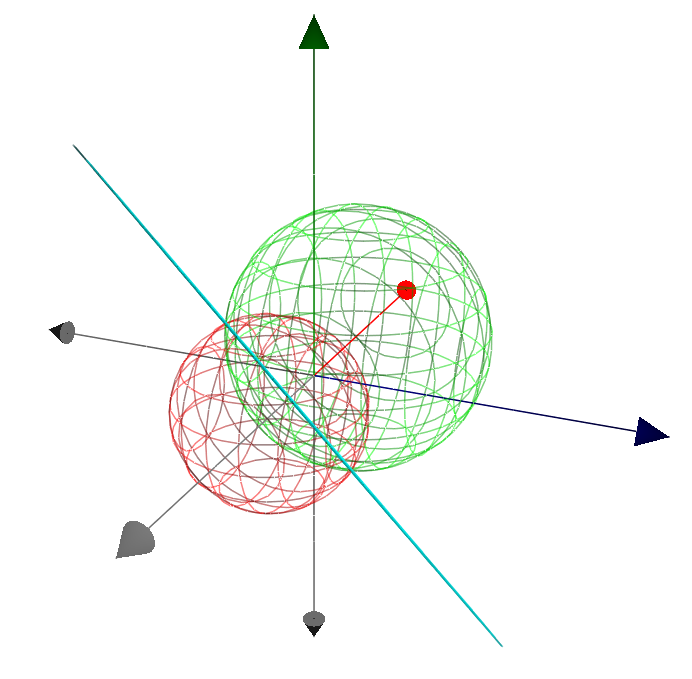
\includegraphics[scale=0.7]{DiffOfSpheres}
\caption{The difference of two spheres gives a plane, shown here on edge.  The spheres were rendered as a number of traces in various parallel planes.}
\label{fig_diff_of_spheres}
\end{figure}

At first sight, the sum of a sphere and a plane may not seem that interesting.
However, the sum of a homogenized sphere and a non-homogenized plane is
interesting, because the result is always a sphere in homogenized form.  The
scalar amount at which the plane is non-homogenized simply indicates half
the length along the normal of the plane that the center of the original sphere
is displaced in the direction of that normal to find a sphere intersecting the
plane in the same circle as that of the original sphere.

Interestingly, the difference of spheres generalizes to the idea of subtracting
spheroids.  A picture of this is given in Figure~\ref{fig_diff_of_spheroids}.
Of course, there is undoubtedly a geometric significance in the difference
between any two quadric surfaces.

\begin{figure}
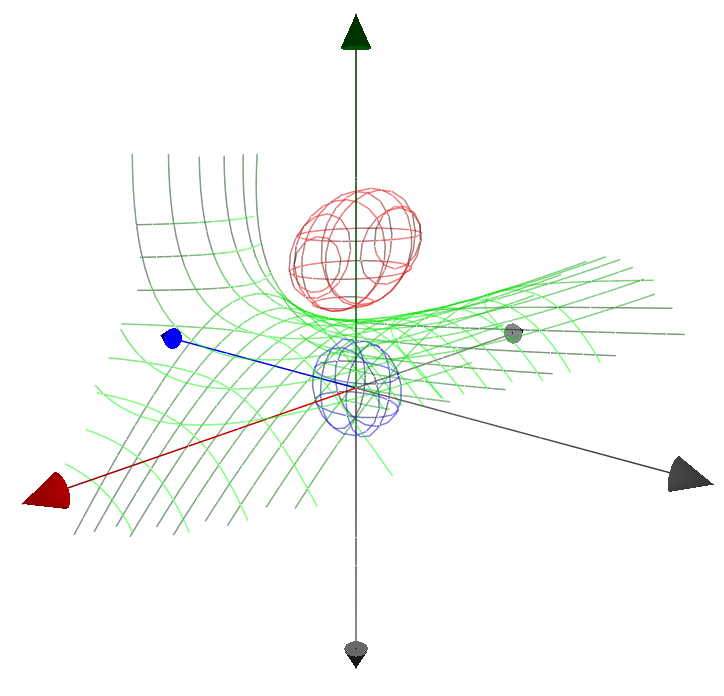
\includegraphics[scale=0.7]{DiffOfSpheroids}
\caption{The difference of two spheroids gives a hyperbolic paraboloid.  Traces in various planes were used to render the surfaces.}
\label{fig_diff_of_spheroids}
\end{figure}


% Can we add a plane to an ellipsoid to find the reflection of the plane in the ellipsoid?

% Note the theorems of CGA that let us do intersections and fittings.
% Show why we can't apply them here.

% Can we get the conic sections?  We just need to intersect planes with quadrics, right?

% lots of use of one def, no results, proofs, theorem?!

\section{A Brief Consideration Of $m$-Vectors}

Specifically, what is meant here is the consideration of $m$-vectors where $m\neq 2$.
What we find in this section, unfortunately, is that such vectors with $m>2$
are unlikely to play an interesting role in the model.  What is immediately
obvious is that for any such $m$-vector $M$, the $(m-2)$-vector
$p\wedge\overline{p}\cdot M$, when set to zero, creates a system
of equations whose solution set is the intersection of all
geometries represented by each individual equation.  The problem with
this is that $M$, as an element of $\G$, does not characterize
this intersection directly, but only indirectly as the characterization
of each individual geometry taken in the intersection.
It follows that no decomposition of $M$ is likely to easily reveal any information
about the intersection that is $M$.  One redeeming idea in all of this, however,
stems from the common theme found throughout various models of geometry as
that of simply going from one characterization of some piece of geometry to another.
While $M$ may not directly characterize the geometry it represents,
it may offer a characterization alternative to the one used in
the formulation of $M$.  And sometimes that is what doing geometry is all about
in models of geometry based in geometric algebra.

To illustrate the point, realize that any trivector $T\in\G$ has the form
\begin{equation}
T = \sum_{i=1}^k v_i\wedge B_i,
\end{equation}
where $\{v_i\}_{i=1}^k\subset\W$ is a set of $k$ vectors and $\{B_i\}_{i=1}^k\subset\G$
is a set of $k$ bivectors.  Applying Definition~\ref{def_quadric}, we get
\begin{equation}\label{equ_trivector_geo}
0 = p\wedge\overline{p}\cdot T =
p\cdot\sum_{i=1}^k(\overline{p}\cdot v_i)B_i -
\overline{p}\cdot\sum_{i=1}^k(p\cdot v_i)B_i +
\sum_{i=1}^k(p\wedge\overline{p}\cdot B_i)v_i.
\end{equation}
Now if $\{v_i\}_{i=1}^k$ was a linearly independent set, and for all point $p\in\V$, we had $p\cdot v_i=\overline{p}\cdot v_i=0$
for any integer $i\in[1,k]$, (which is not possible anyway without expanding the dimension our geometric algebra), then it is clear
from equation \eqref{equ_trivector_geo} that $T$ represents the intersection of all quadrics in $\{B_i\}_{i=1}^k$.  Now while this
may be true, $T$ certainly does not characterize the intersection directly, but only indirectly through the characterizations
of each $B_i$.  This result is therefore useless unless perhaps the formulation of $T$ was made through some means other than that of
taking the intersection of the $B_i$ quadrics.  But as pointed out, this condition cannot be satisfied in $\G$, so it may, in any case,
be interesting to formulate trivectors this way, and see what we get.

As for any vector $v\in\W$, under Definition~\ref{def_quadric} this represents the set of all
projective points $p$ such that $0=\overline{p}\cdot v$.  Clearly, only those vectors $v$ found
in the complement of $\V$ with respect to $\W$ will hold any interest for us.

\section{Transformations In The Model}

Explore the idea of applying versors to bivectors here.

% What about transformations?

\section{Concluding Remarks}

That $\G$ was not something fancy like a Minkowski space or some other
type of non-Euclidean geometric algebra was perhaps our first clue from
the beginning that the potential for great things coming out of this model
was, let's say, less than likely.  On the other hand, it is very hard to see
all ends, and so perhaps there are deep results to be found or new insights
to be had using this method of studying quadric surfaces.  In any case,
geometric algebra has proven to be a fundamental, versatile and unifying
language that perhaps most naturally extends mathematics beyond the real number line.  Perhaps
there is a much better way to use geometric algebra to study quadric surfaces.

While it has been shown that elements of $\G$ do indeed, under a given
definition, represent quadric surfaces, there really is nothing more or less
interesting about adding and subtracting these elements than adding and
subtracting vector equations whose solution sets represent the quadric surfaces.
There might not be any advantage in using the elemental form over the
functional form.

% Another problem is that, unlike CGA, we're not using blades exclusively.
% if we were, then we wouldn't run into the addition/intersection problem.

%    Bibliographies can be prepared with BibTeX using amsplain,
%    amsalpha, or (for "historical" overviews) natbib style.
\bibliographystyle{amsplain}
%    Insert the bibliography data here.

\bibliography{Parkin_QuadricSurfacesUsingGA}

\end{document}

%%%%%%%%%%%%%%%%%%%%%%%%%%%%%%%%%%%%%%%%%%%%%%%%%%%%%%%%%%%%%%%%%%%%%%%%

%    Templates for common elements of a journal article; for additional
%    information, see the AMS-LaTeX instructions manual, instr-l.pdf,
%    included in the ECGD author package, and the amsthm user's guide,
%    linked from http://www.ams.org/tex/amslatex.html .

%    Section headings
\section{}
\subsection{}

%    Ordinary theorem and proof
\begin{theorem}[Optional addition to theorem head]
% text of theorem
\end{theorem}

\begin{proof}[Optional replacement proof heading]
% text of proof
\end{proof}

%    Figure insertion; default placement is top; if the figure occupies
%    more than 75% of a page, the [p] option should be specified.
\begin{figure}
\includegraphics{filename}
\caption{text of caption}
\label{}
\end{figure}

%    Mathematical displays; for additional information, see the amsmath
%    user's guide, linked from http://www.ams.org/tex/amslatex.html .

% Numbered equation
\begin{equation}
\end{equation}

% Unnumbered equation
\begin{equation*}
\end{equation*}

% Aligned equations
\begin{align}
  &  \\
  &
\end{align}

%-----------------------------------------------------------------------
% End of ecgd-l-template.tex
%-----------------------------------------------------------------------
